\chapter{Medida del rendimiento y perfilado}
\label{chap:medida_rendimiento_perfilado}

\lettrine{E}{n} este capítulo, tras plantear la problemática y documentar cómo se construye la prueba de concepto en los capítulos anteriores, se muestran los resultados de las medidas de rendimiento tanto para los códigos densos como dispersos, tanto basados en librería como en arquitectura punto a punto. Estos resultados se comparan con los que se pueden ver en la literatura ya existente, para comprobar si la red implementada se adhiere a los patrones indicados, por ejemplo, en la Sección \ref{sec:investigacion_optimizaciones_propuestas}.

\section{Metodología}
\label{sec:metodologia}
La medida del rendimiento de las pruebas de concepto se realiza por partes mediante el empleo del reloj monotónico del sistema en microsegundos. Al ser sobre todo los códigos densos y de librería simples pruebas de concepto, funciones auxiliares como por ejemplo \texttt{map\_and\_bias} no está debidamente paralelizada con OpenMP, a diferencia de la versión punto a punto, donde realizar esto es tarea trivial partiendo de la base de que OpenMP ya es necesario para el funcionamiento base. Realizar esta optimización no es difícil, es algo innecesario cuando lo que se pretende es medir las posibilidades de una aproximación, centrándose en el producto de matrices, y no optimizar y trabajar a fondo con una implementación en particular.

Por esta razón se ha decidido simplemente implementar de forma sencilla la generación de código con las librerías \texttt{OpenBLAS} y \texttt{librsb} sin añadir OpenMP, y la punto a punto completamente paralelizada con OpenMP. El \textit{overhead} que añade el procesado auxiliar de datos de forma secuencial es creciente conforme se aumentan el número de procesadores paralelos. Sin embargo, debido a que las mediciones de tiempos se realizan de forma aislada, estas no precisan de paralelización en un entorno de pruebas.

\subsection{Común}
\label{ssec:comun_metodologia}
Para la medida del rendimiento y perfilado se generan dos redes neuronales de un tamaño absurdamente grande, una densa con capas completamente conexas con un anchos tal que \{capa de entrada, $n\:\times\:$capas ocultas, capa de salida\} = \{24, 500, 800, 1000, 1200, 600, 400, 200, 100, 50, 1\}, y varias redes dispersas basadas en esta primera, con índices de dispersión del 60\%, 70\%, 80\%, 85\%, 90\%, 95\% y 99\%. Evidentemente, para el problema que se pretende resolver, estas redes están completamente sobredimensionadas y son cuanto menos inútiles, puesto que debido a su enorme tamaño lo único que aprenden durante el proceso de entrenamiento es a marcar como positivos todos los \textit{inputs}.

Esto, que para un ingeniero en inteligencia artificial sería un enorme fracaso, en este ámbito es algo completamente indiferente, ya que a pesar de la inutilidad de la red creada, ésta sigue realizando las cargas de trabajo típicas de una red neuronal adecuada. Esto es, la red tiene que multiplicar matrices, sumar los \textit{bias} y aplicar las funciones de transferencia.

En todas las ejecuciones se emplean los mismos datos de entrada replicados $n$, basados en el fichero \texttt{input.txt} generado con la función tratada en el Punto 3 de la Sección \ref{ssec:extraccion_valores}. En concreto, estos datos se replican 100 y 1000 veces, para obtener $1000 \times 100 = 100000$ y $1000 \times 1000 = 1000000$ datos de entrada.

\subsection{Medida del rendimiento}
\label{ssec:medida_rendimiento_metodologia}
Para la medida del rendimiento se emplea el reloj monotónico del sistema mediante la función \texttt{clock\_gettime(CLOCK\_MONOTONIC\_RAW, \&timestamp)} en compilaciones de \textit{release} (opción \texttt{-s} o \textit{strip}). Se realizan cinco ejecuciones para cada red y \textit{sparsity}, y se guarda la salida de \texttt{stdout} con el script \texttt{run\_tests.sh}:\medskip
\begin{lstlisting}[language=bash]
#!/bin/sh
mkdir -p logs
INPUT=inputs/input_long.txt

for it in 1 2 3 4 5; do
./dense.out $INPUT > logs/dense.$it.log
for sp in 60 70 80 85 90 95 99; do
    echo RUNNING LIBRSB FOR $sp% SPARSITY $it ITERATION
    ./sparse_$sp.out $INPUT > logs/sparse_$sp.$it.log

    echo RUNNING P2P FOR $sp% SPARSITY $it ITERATION
    ./p2p_$sp.out $INPUT > logs/p2p_$sp.$it.log
done
done  
\end{lstlisting}

Las ejecuciones para medición de tiempos se realizan en la partición \texttt{compute2} del clúster Plutón\footnote{\url{https://pluton.dec.udc.es/guide/user-guide.pdf}}, con características visibles en la Tabla \ref{tb:especificaciones_compute2}. Los perfilados, sin embargo, se realizan en un equipo Xiaomi Mi Notebook 15 con las características visibles en la Tabla \ref{tb:especificaciones_xiaomi}.
\begin{table}
    \centering
    \begin{tabular}{|c|c|}
        \hline
        CPU & 2x Intel Xeon Silver 4216 (2x16C/32T) @ 3.2GHz\\\hline
        RAM & 256GB DDR4 2933Mhz (8 $\times$ 32GB)\\\hline
        Sistema & CentOS Linux release 7.9.2009 (Core) \\\hline
        Kernel & 3.10.0-1160.76.1.el7.x86\_64 \\\hline
        CC & gcc 9.3.0\\\hline
        OpenBLAS & OpenBLAS 0.3.21\\\hline
        librsb & librsb 1.3.0.1\\\hline
    \end{tabular}
    \caption{\label{tb:especificaciones_compute2}Especificaciones técnicas de un equipo en la partición \texttt{compute2} del clúster Plutón}
    \end{table}

\begin{table}
\centering
\begin{tabular}{|c|c|}
    \hline
    CPU & 11th Gen Intel Core i7-11370H (4C/8T) @ 3.3GHz\\\hline
    RAM & 16GB DDR4 3200MHz (\textit{Row-of-chips} {\small$\approx$} 2 $\times$ 8GB)\\\hline
    Sistema & Ubuntu 20.04.5 LTS\\\hline
    Kernel & 5.15.0-50-generic \\\hline
    CC & gcc 9.4.0\\\hline
    OpenBLAS & OpenBLAS 0.3.21\\\hline
    librsb & librsb 1.3.0.1\\\hline
    oneAPI & Intel oneAPI 2022.3\\\hline
\end{tabular}
\caption{\label{tb:especificaciones_xiaomi}Especificaciones técnicas del Xiaomi Mi Notebook 15}
\end{table}


\subsection{Análisis y perfilado}
\label{ssec:analisis_perfilado_metodologia}
Para el análisis y perfilado se emplea el programa Intel Advisor, el cual permite realizar modelos \textit{roofline} de partes individualizadas de programas, incluyendo las funciones de su librería \acrshort{mkl} (\textit{\acrlong{mkl}}). Esto es especialmente útil para perfilar tanto la implementación densa, que emplea funciones de \texttt{cblas} ampliamente utilizadas, así como la punto a punto, que no emplea ninguna llamada a librería.

Sin embargo, esta universalidad se pierde con la versión dispersa (\textit{sparse}), ya que se emplean funciones \textit{built-in} de \texttt{OpenBLAS}, así como funciones propias de \texttt{librsb}, lo que hace que cambiar a la \acrshort{mkl} requiera una reprogramación de ciertas líneas del código para poder perfilar las funciones de librería con Intel Advisor. Esto es algo costoso que inicialmente puede parecer un problema, pero es un trabajo que se puede evitar si se razona con respecto al modelo \textit{roofline} de la versión densa.

\subsection{Compilación}
\label{ssec:compilacion_metodologia}
Para compilar las versiones densa y dispersa se requiere intercambiar \texttt{OpenBLAS} por la Intel \acrshort{mkl}, así como desactivar el \textit{stripping} del binario para activar los símbolos de depuración (susituir parámetro \texttt{-s} por \texttt{-g}). La versión punto a punto no requiere modificaciones significativas ya que únicamente emplea librerías estándar. En cuanto a las funciones de \acrshort{blas}, la modificación de las líneas de compilación genéricas que se pueden encontrar en el fichero \texttt{.ipynb} se muestra estructurado a continuación.

\subsubsection{Código denso}
Para la obtención del \textit{roofline model} de la carga de trabajo, es necesario o bien calcularlo manualmente, o bien emplear alguna herramienta adecuada para ello. Como ya se comenta previamente, se emplea Intel Advisor para el perfilado del código, por lo que es necesario compilar el código denso con una configuración que sustituya \texttt{OpenBLAS} por \acrshort{mkl}. Para esto se puede compilar de las siguientes formas:\medskip
\begin{lstlisting}[language=bash]
# Para una compilación convencional sin depuración con OpenBLAS, sería necesario únicamente ejecutar
gcc -march=native -O3 -s common.c dense.c -o dense.out -lm -lopenblas

# Sin embargo, con propósitos de perfilado con Intel Advisor, en un entorno bash donde se haya realizado `source /opt/intel/oneapi/setvar.sh` se ha de compilar con:
gcc -march=native -O3 -g3 -DMKL_ILP64 -m64 -I"${MKLROOT}/include" common.c dense.c -o dense.out -L${MKLROOT}/lib/intel64 -Wl,--no-as-needed -lmkl_intel_ilp64 -lmkl_gnu_thread -lmkl_core -lgomp -lpthread -lm -ldl
\end{lstlisting}

\subsubsection{Código \textit{sparse}}
En este caso, debido al uso de \texttt{librsb} como librería de Sparse BLAS, la herramienta de perfilado y análisis de código Intel Adviso no es capaz de analizar el código de librerían ni compilando la misma con flags de \textit{debug}. Como se comenta previamente, una adaptación a la librería Intel MKL, a pesar de no ser imposible, no es conveniente. Por esto mismo más adelante en este capítulo se estima el rendimiento y posibilidades de mejora del código disperso, en función a los resultados con respecto al denso. Para compilar el código para \textit{release}, las líneas de compilación son las siguientes:\medskip
\begin{lstlisting}[language=bash]
# Para una compilación convencional sin depuración con OpenBLAS, sería necesario únicamente ejecutar
gcc -march=native -O3 -s common.c dense.c -o sparse.out -lm -lrsb -lopenblas
\end{lstlisting}

\subsubsection{Código \textit{point-to-point}}
En este caso solamente se emplean librerías estándar, por lo que para GCC, en las líneas de compilación simplemente se cambia \texttt{-s} por \texttt{-g3}. Por otro lado y debido a que en este caso la optimización del compilador si es algo importante, ya que no se emplean únicamente funciones de librería, también se emplean los dos compiladores de Intel, que son el antiguo ICC y el nuevo ICX, basado en LLVM\footnote{Documentación empleada para compilación, así como para posibles líneas de optimización futura, están disponibles en \url{https://www.intel.com/content/www/us/en/developer/articles/guide/porting-guide-for-icc-users-to-dpcpp-or-icx.html}.}:\medskip
\begin{lstlisting}[language=bash]
# Para una compilación con OpenMP
gcc -march=native -O3 -g3 common.c p2p.c -o p2p.out -lm -fopenmp

# Para una compilación sin OpenMP
gcc -march=native -O3 -g3 common.c p2p.c -o p2p.out -lm -fno-openmp

# Además, para comparación con Intel ICC (Legacy)
icc -xHost -O3 -g3 common.c p2p.c -o p2p.out -lm -qopenmp
# Y con el nuevo compilador ICX basado en LLVM
icx -xhost -O3 -g3 common.c p2p.c -o p2p.out -lm -fiopenmp
\end{lstlisting}

\section{Medida de rendimiento}
\label{sec:medida_rendimiento}
En esta sección se muestra una comparación de rendimientos entre las diferentes implementaciones o \textit{\gls{backend}s} para cada \textit{sparsity} y aproximación usada (\texttt{OpenBLAS}, \texttt{librsb} o p2p), basados en medidas obtenidas según la metodología descrita en la sección anterior.

En primer lugar, en la Figura \ref{fig:rendimiento_100k} se muestran los resultados para 100k datos de entrada. En ésta se puede observar como la aproximación punto a punto supera ampliamente a \texttt{OpenBLAS} a partir del 87,5\% de \textit{sparsity}, mientras que \texttt{librsb} no es capaz de superar a \texttt{OpenBLAS} en ningún caso, lo que quizás indique que esta librería está enfocada a matrices con un índice de dispersión mayor.

En la Figura \ref{fig:rendimiento_1M} se pueden observar resultados muy similares, destacando quizás que acercándose a índices mayores de dispersión el código mejora mucho más que con una cantidad de datos inferior. Este comportamiento se puede apreciar más claramente en la Figura \ref{fig:cross_speedup_1M_100k}, donde se analiza el \textit{cross-speedup} entre la Figura \ref{fig:rendimiento_100k} y la Figura \ref{fig:rendimiento_1M}. Esto es, siendo $XS(A/B)$ el \textit{cross-speedup}, $S(A)$ y $S(B)$ el speedup obtenido con $A$ y $B$ elementos, respectivamente, se puede decir que la magnitud que se representa gráficamente se calcula tal que:
\begin{equation}
    XS(1M/100k) = S(1M) / S(100k)\nonumber
    \label{eq:cross_speedup}
\end{equation}

Así, se puede apreciar que la mejoría del speedup con un dataset 10 veces más grande es cada vez más alta a partir del 90\% de \textit{sparsity} para la implementación punto a punto, siendo sin embargo inferior el rendimiento basado en \texttt{librsb}.

\begin{figure}[htpb]
\centering
\begin{tikzpicture}
    \begin{axis}[
        xmin = 55, xmax = 105, xlabel=\textit{sparsity},
        ymin = 0.01, ymax=19, ymode=log, log basis y=10, ylabel=\textit{speedup}, yticklabels={PADDING, {0,01}, {0,1}, 1, 10},
        width = \textwidth,
        height = 0.55\textwidth,
        grid=both,
        legend pos=north west,
    ]

    \addplot[udcgray,smooth,very thick,mark=*] coordinates {
        (60,1)
        (70,1)
        (80,1)
        (85,1)
        (90,1)
        (95,1)
        (99,1)
    };
    \addlegendentry{OpenBLAS}
    
    \addplot[ficblue,smooth,very thick,mark=*] coordinates {
        (60,0.042)
        (70,0.055)
        (80,0.074)
        (85,0.094)
        (90,0.127)
        (95,0.204)
        (99,0.511)
    };
    \addlegendentry{librsb}

    \addplot[udcpink,smooth,very thick,mark=*] coordinates {
        (60,0.262)
        (70,0.361)
        (80,0.574)
        (85,0.806)
        (90,1.253)
        (95,2.852)
        (99,9.985)
    };
    \addlegendentry{p2p}

    % Kinda ugly
    % \vasymptote[udcpink]{87.72}
    \end{axis}
\end{tikzpicture}
\caption{Speedups según \textit{sparsity} para 100k datos de entrada}
\label{fig:rendimiento_100k}
\end{figure}

\begin{figure}[htpb]
    \centering
    \begin{tikzpicture}
        \begin{axis}[
            xmin = 55, xmax = 105, xlabel=\textit{sparsity},
            ymin = 0.01, ymax=19, ymode=log, log basis y=10, ylabel=\textit{speedup}, yticklabels={PADDING, {0,01}, {0,1}, 1, 10},
            width = \textwidth,
            height = 0.55\textwidth,
            grid=both,
            legend pos=north west,
        ]
    
        \addplot[udcgray,smooth,very thick,mark=*] coordinates {
            (60,1)
            (70,1)
            (80,1)
            (85,1)
            (90,1)
            (95,1)
            (99,1)
        };
        \addlegendentry{OpenBLAS}
        
        \addplot[ficblue,smooth,very thick,mark=*] coordinates {
            (60,0.037)
            (70,0.050)
            (80,0.069)
            (85,0.087)
            (90,0.120)
            (95,0.201)
            (99,0.550)
        };
        \addlegendentry{librsb}
    
        \addplot[udcpink,smooth,very thick,mark=*] coordinates {
            (60,0.289)
            (70,0.399)
            (80,0.629)
            (85,0.850)
            (90,1.367)
            (95,3.352)
            (99,15.694)
        };
        \addlegendentry{p2p}
        \end{axis}
    \end{tikzpicture}
    \caption{Speedups según \textit{sparsity} para 1M de datos de entrada}
    \label{fig:rendimiento_1M}
\end{figure}

\begin{figure}[htpb]
    \centering
    \begin{tikzpicture}
        \begin{axis}[
            xmin = 55, xmax = 105, xlabel=\textit{sparsity},
            ymin = 0.8, ymax=1.7, ylabel=\textit{cross-speedup},
            width = \textwidth,
            height = 0.55\textwidth,
            grid=both,
            legend pos=north west,
        ]
    
        \addplot[udcgray,smooth,very thick,mark=*] coordinates {
            (60,1)
            (70,1)
            (80,1)
            (85,1)
            (90,1)
            (95,1)
            (99,1)
        };
        \addlegendentry{OpenBLAS}
        
        \addplot[ficblue,smooth,very thick,mark=*] coordinates {
            (60,0.879)
            (70,0.911)
            (80,0.928)
            (85,0.925)
            (90,0.942)
            (95,0.985)
            (99,1.076)
        };
        \addlegendentry{librsb}
    
        \addplot[udcpink,smooth,very thick,mark=*] coordinates {
            (60,1.105)
            (70,1.104)
            (80,1.096)
            (85,1.054)
            (90,1.091)
            (95,1.175)
            (99,1.572)
        };
        \addlegendentry{p2p}
        \end{axis}
    \end{tikzpicture}
    \caption{Cross-speedup según \textit{sparsity} de 1M con respecto a 100k datos de entrada}
    \label{fig:cross_speedup_1M_100k}
\end{figure}

\section{Perfilado y \textit{roofline model}}
\label{sec:perfilado_roofline}
En esta sección se muestran las características de cada carga de trabajo con ayuda de Intel Advisor, y se razonan los posibles resultados que no se han podido obtener debido a limitaciones en el análisis.

\subsection{Código denso}
Los resultados obtenidos para la red neuronal densa son, tal como se espera de una librería de BLAS de amplio uso como \texttt{OpenBLAS}, excelentes. Estos resultados se obtienen además realizando un excelente uso de la memoria caché, y tal como se muestra en el modelo \textit{roofline} en la Figura \ref{fig:roofline_dense}, los resultados obtiene la Intel MKL son extrapolables por similitud en los tiempos a los de \texttt{OpenBLAS}.

\begin{figure}[h!]
    \centering
    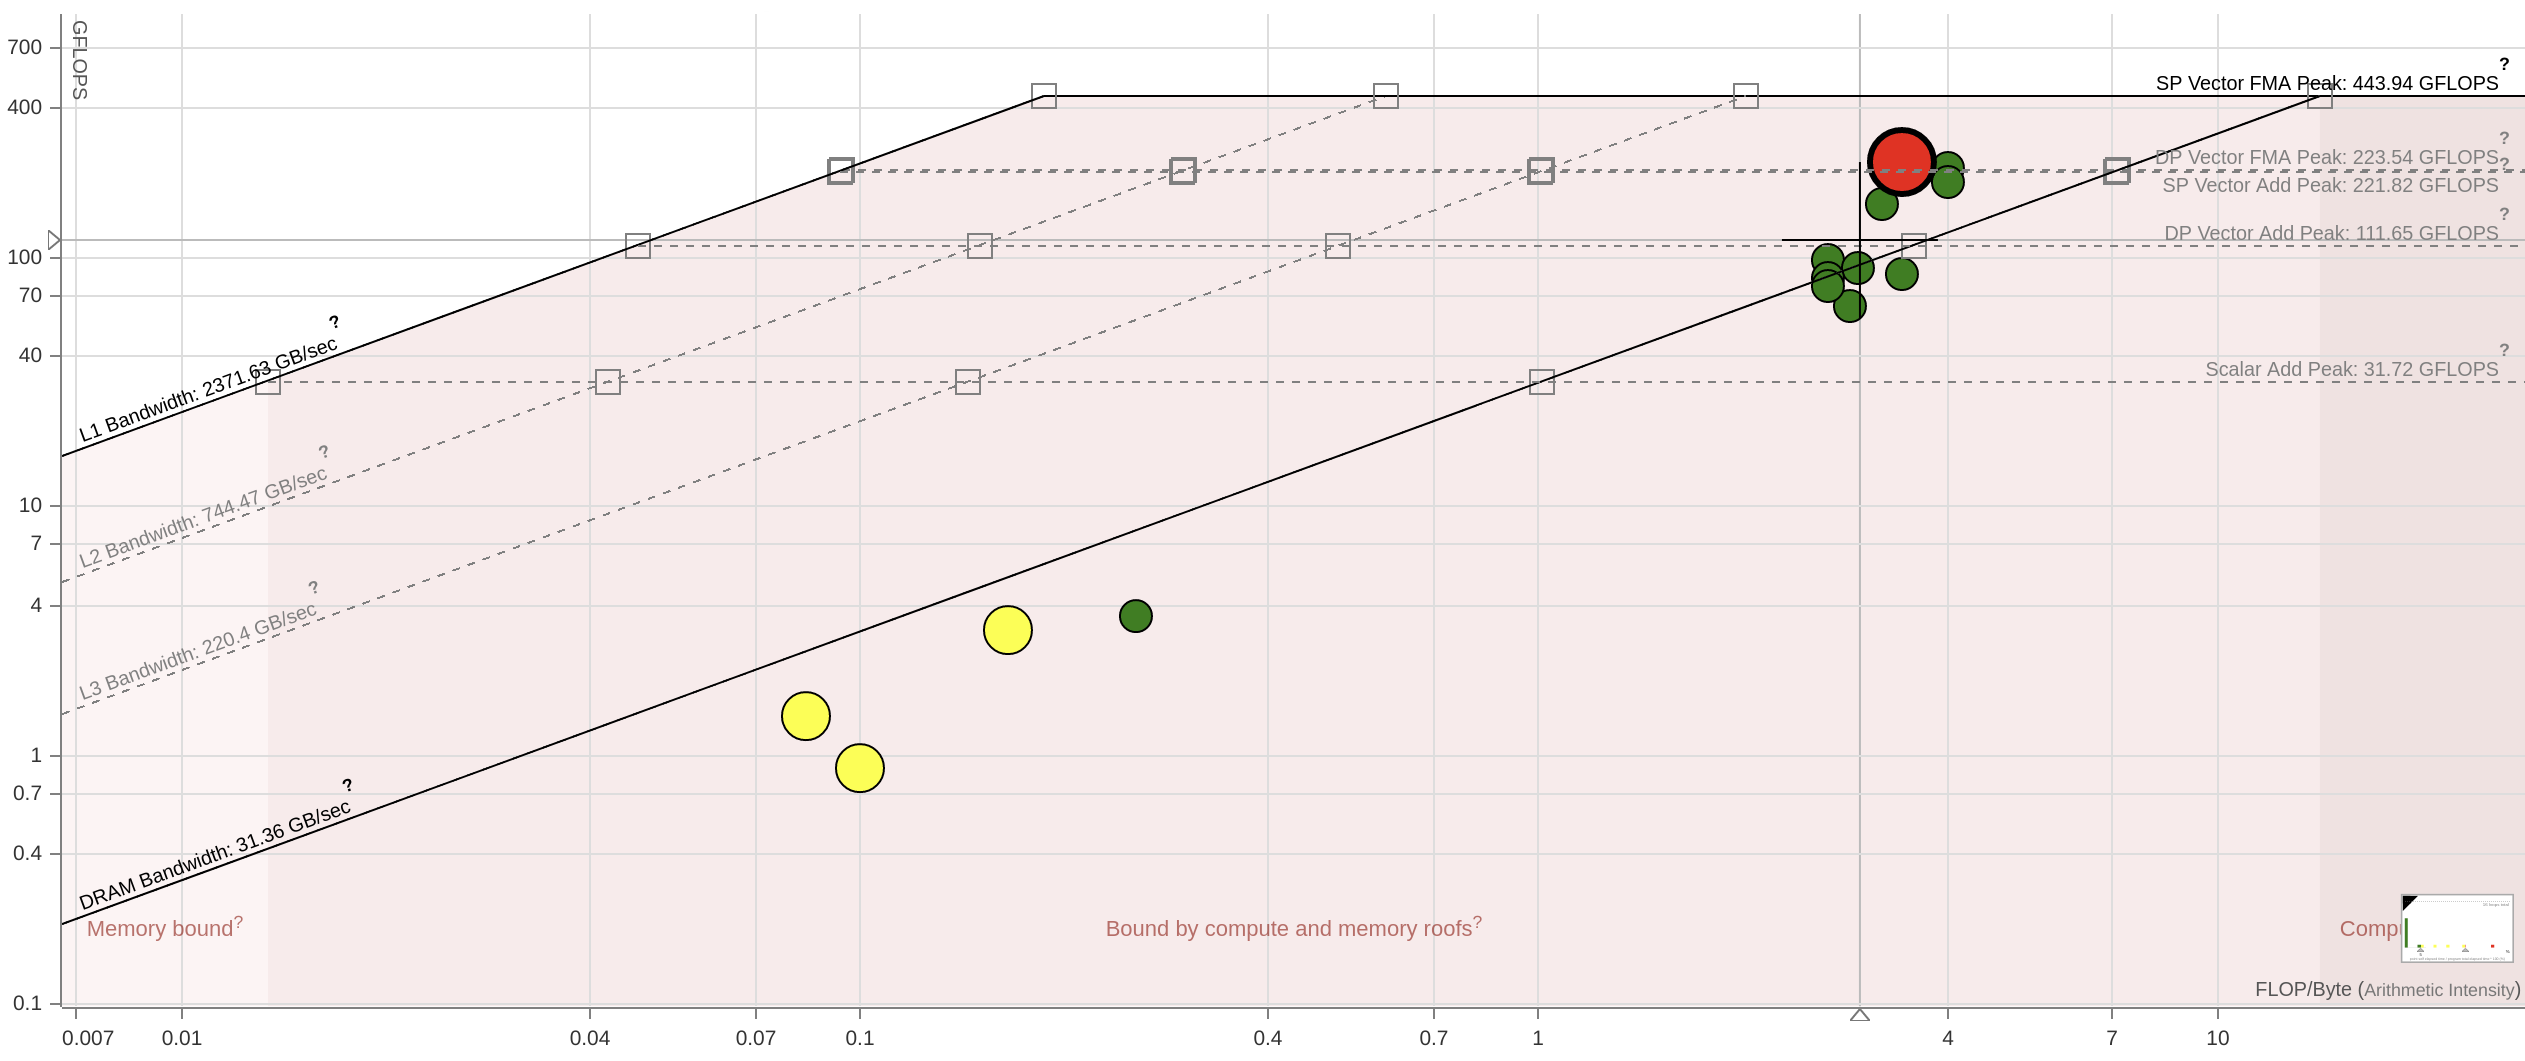
\includegraphics[width=\textwidth]{img/rooflines/roofline_dense.png}
    \caption{\textit{Roofline model} del código denso}
    \label{fig:roofline_dense}
\end{figure}

Como se puede apreciar en el modelo, el \textit{workload} de interés, que es el que se puede encontrar en la parte superior derecha (coloreado en rojo y verde), corresponde a las funciones \texttt{cblas\_sgemm}. Estas funciones están fuertemente optimizadas y emplean instrucciones AVX512, como se puede observar en los detalles de la carga (Figura \ref{fig:roofline_dense_details}).

Fijándose con atención se pueden ver funciones con un considerablemente menor desempeño en la parte inferior izquierda. Estos puntos corresponden a \texttt{map\_and\_bias} y sucesivas llamadas a otras funciones como \texttt{expf}. Tal como se comenta previamente, una paralelización de funciones auxiliares es sencilla. Sin embargo, y tal como se puede ver en el modelo, se pueden distinguir perfectamente los componentes de dichas funciones, por lo que es sencillo discernir qué mejorías podrían ser obtenidas mediante un cambio en el producto de matrices más eficiente.    

\begin{figure}[h!]
    \centering
    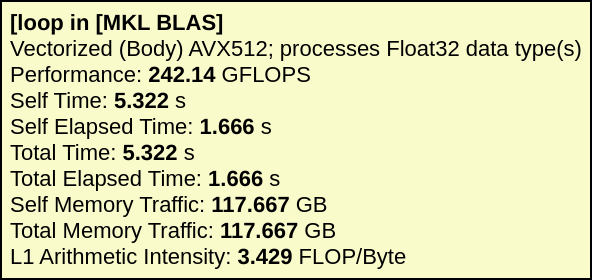
\includegraphics[width=0.5\textwidth]{img/rooflines/roofline_dense_details.png}
    \caption{Detalles de \texttt{cblas\_sgemm} en el modelo del código denso}
    \label{fig:roofline_dense_details}
\end{figure}

\subsection{Código \textit{sparse}}
Por otro lado, los resultados obtenidos para la red neuronal dispersa, y tal como se comenta previamente, algo decepcionantes. En este caso, debido al empleo de la librería \texttt{librsb}, el modelo \textit{roofline} no contiene información de utilidad (Figura \ref{fig:roofline_sparse_details}). Esto, que a todas luces es un problema, deja de serlo si se realiza un sencillo razonamiento.

\begin{figure}[h!]
    \centering
    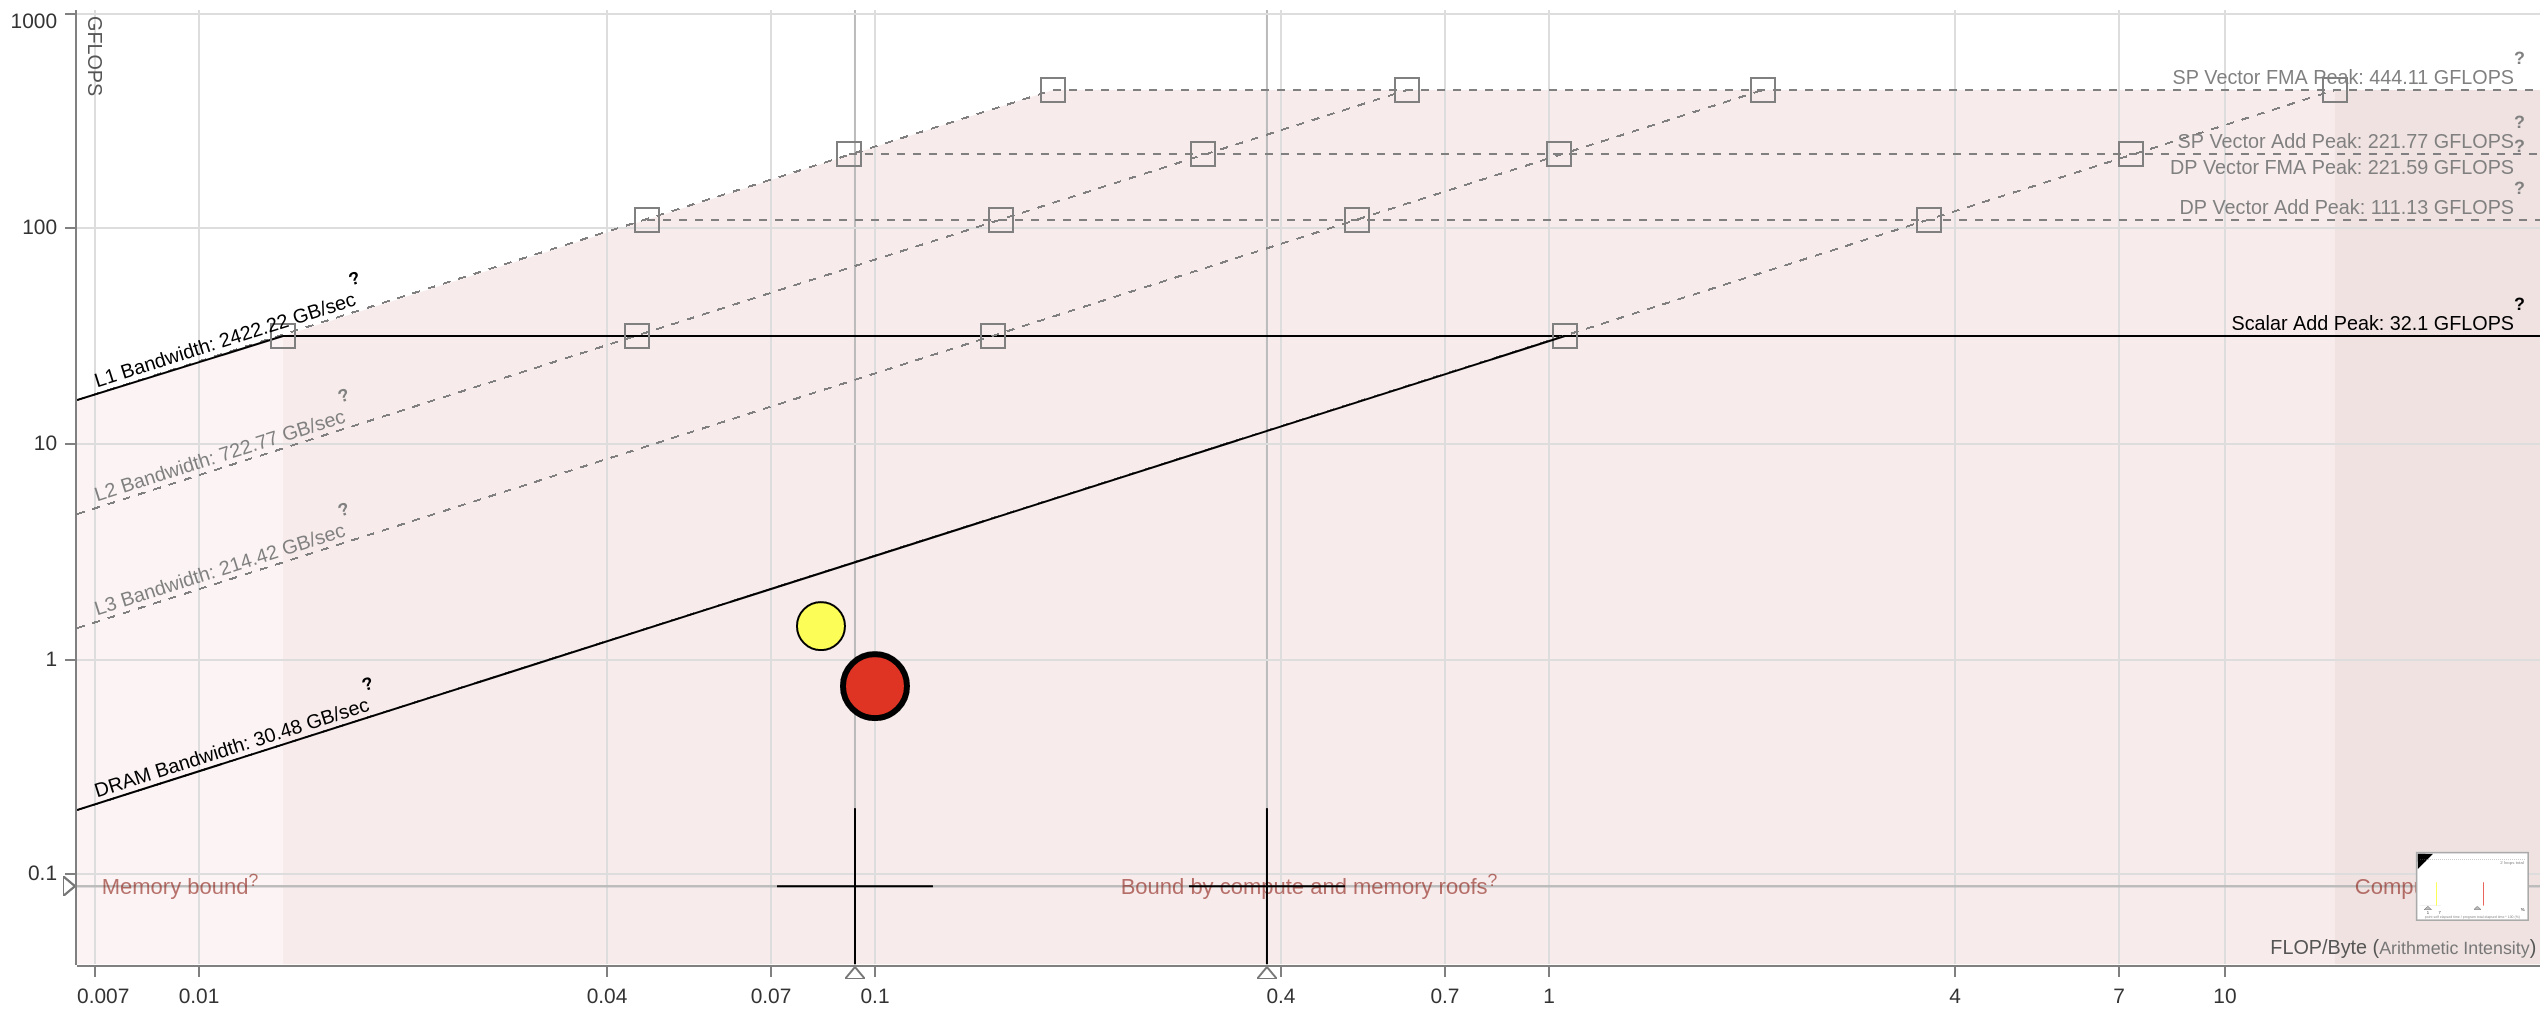
\includegraphics[width=\textwidth]{img/rooflines/roofline_sparse.png}
    \caption{\textit{Roofline model} del código disperso}
    \label{fig:roofline_sparse_details}
\end{figure}

Teniendo en cuenta que los tiempos de ejecución de una red dispersa al 95\% son 5 veces superiores a los de la red completamente conexa aún teniendo que procesar un 95\% menos de datos, se puede realizar una estimación del número teórico de FLOP necesarios para las operaciones de multiplicación.

\subsubsection{Aproximación teórica}
Tal como se explica en la Sección \ref{sec:multiplicacion_point_to_point}, teniendo en cuenta que una operación FMA realiza dos FLOP, se puede concluir que el número de FLOP para la multiplicación de dos matrices $d\times D$ será $2 \cdot \#nz \cdot k$.

\subsubsection{Estimación del rendimiento}
Teniendo en cuenta que las matrices dispersas de pesos en el código disperso tienen una densidad del 5\% (o lo que es lo mismo, una \textit{sparsity} del 95\%), desde un punto de vista teórico se puede concluír que se deberían realizar un 95\% menos de operaciones en punto flotante.

Esta reducción en el número de operaciones necesarias, debido a múltiples factores como el principio de localidad, estructura interna a la hora de almacenar la matriz, estructuras de control, así como optimizaciones internas de la propia librería, no se corresponde con una disminución del tiempo de ejecución, sino más bien todo lo contrario. Esta reducción en el número de FLOPS no parece a primera vista ser causado por en un descenso en la intensidad aritmética, puesto que también se cuenta con una cantidad proporcionalmente menor de bytes de datos. Sin embargo, hay que tener en cuenta que para cada valor de cada matriz, se cargan como mínimo dos índices enteros que representan su posición, disminuyendo la intensidad aritmética como mínimo a un tercio. Esto implica reducir el valor en el eje $x$ del modelo \textit{roofline} en un factor de 3.

Por otro lado, sabiendo que se leen un 95\% menos de valores en coma flotante, pero que se tarda cinco veces más, esto repercute en un descenso de $5/0,05=100$ veces en FLOPS (es decir, un descenso a la centésima parte, o dos órdenes de magnitud, en el eje $y$).

Por esta razón, el modelo \textit{roofline} resultante, que el programa Intel Advisor es incapaz de generar por emplear una librería externa, se vería similar a lo que se puede observar en la Figura \ref{fig:roofline_sparse_estimado}.

\begin{figure}[h!]
    \centering
    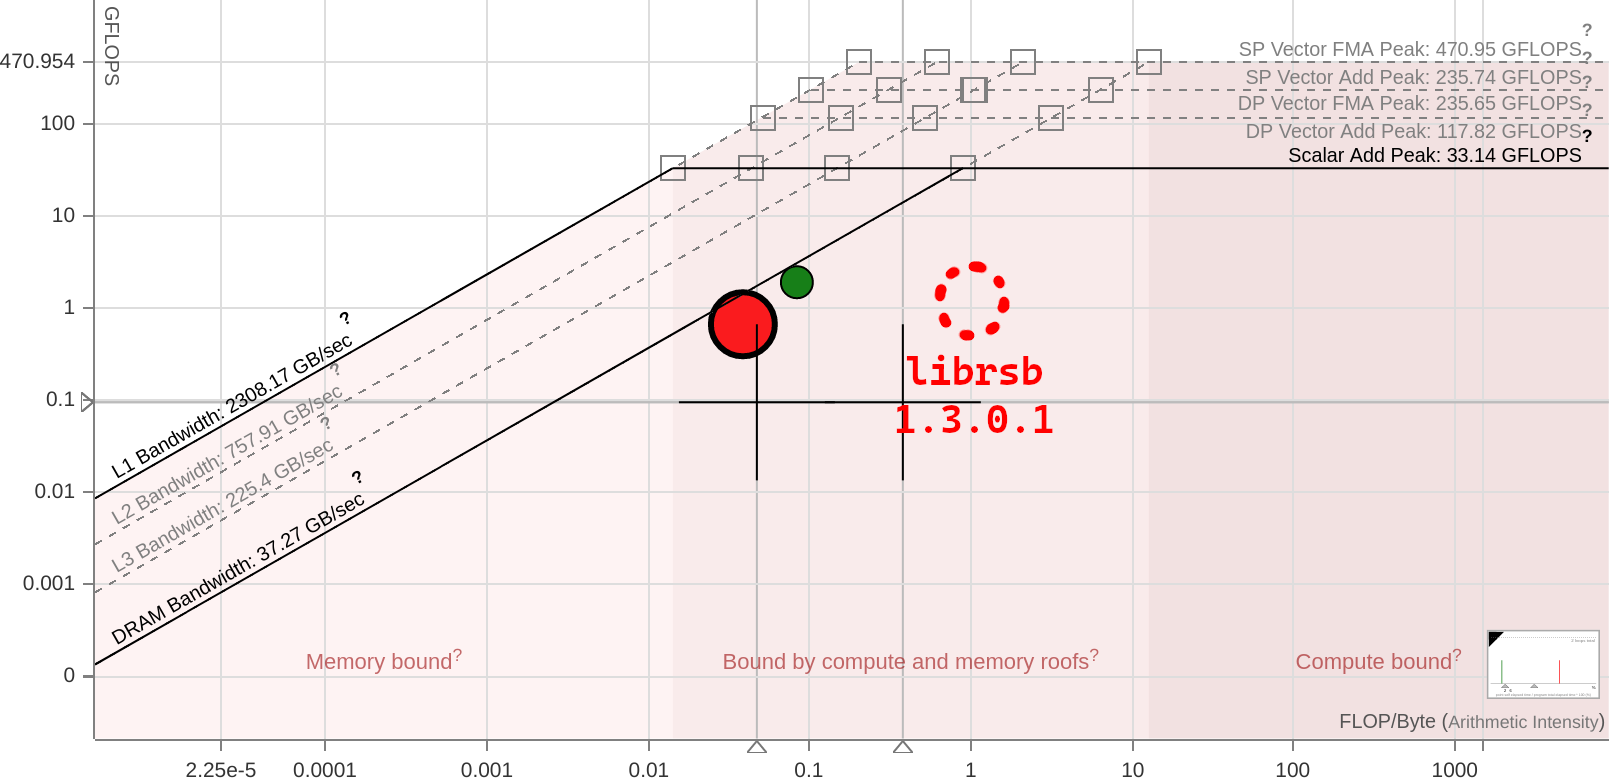
\includegraphics[width=\textwidth]{img/rooflines/roofline_sparse_estimado.png}
    \caption{Estimación del \textit{roofline model} del código disperso}
    \label{fig:roofline_sparse_estimado}
\end{figure}

Estos decepcionantes resultados, sin embargo, motivan la creación de arquitecturas punto a punto, ya que implica que existe un amplio margen de mejora mediante análisis estático de código y generación de instrucciones \textit{ad-hoc}, tanto FMA como de control.


\subsection{Código \textit{point-to-point}}
El código punto a punto es mucho más demandante a nivel de caché de instrucciones, así como en análisis estático de código, con tiempos de compilación que se acercan a las 24 horas y decenas de gigabytes de memoria RAM empleada durante el proceso de optimización. Esta aproximación, sin embargo, debido a lo que se presenta a continuación, se espera que tenga un amplio margen de mejora, siendo posible vectorizar y reordenar gran parte de las instrucciones mediante el empleo de la herramienta MACVETH\footnote{\url{https://github.com/UDC-GAC/MACVETH}}.

\subsubsection{Compiladores empleados}
Para la generación de código punto a punto, se emplean los compiladores de Intel, ICC e ICX, y el compilador GCC, tal como se comenta en la Subsección \ref{ssec:compilacion_metodologia}.

\subsubsection{\textit{Roofline models}}
Para la misma red que en los códigos anteriores, con GCC, se obtiene el modelo visible en la Figura \ref{fig:roofline_p2p_gcc}.
\begin{figure}[h!]
    \centering
    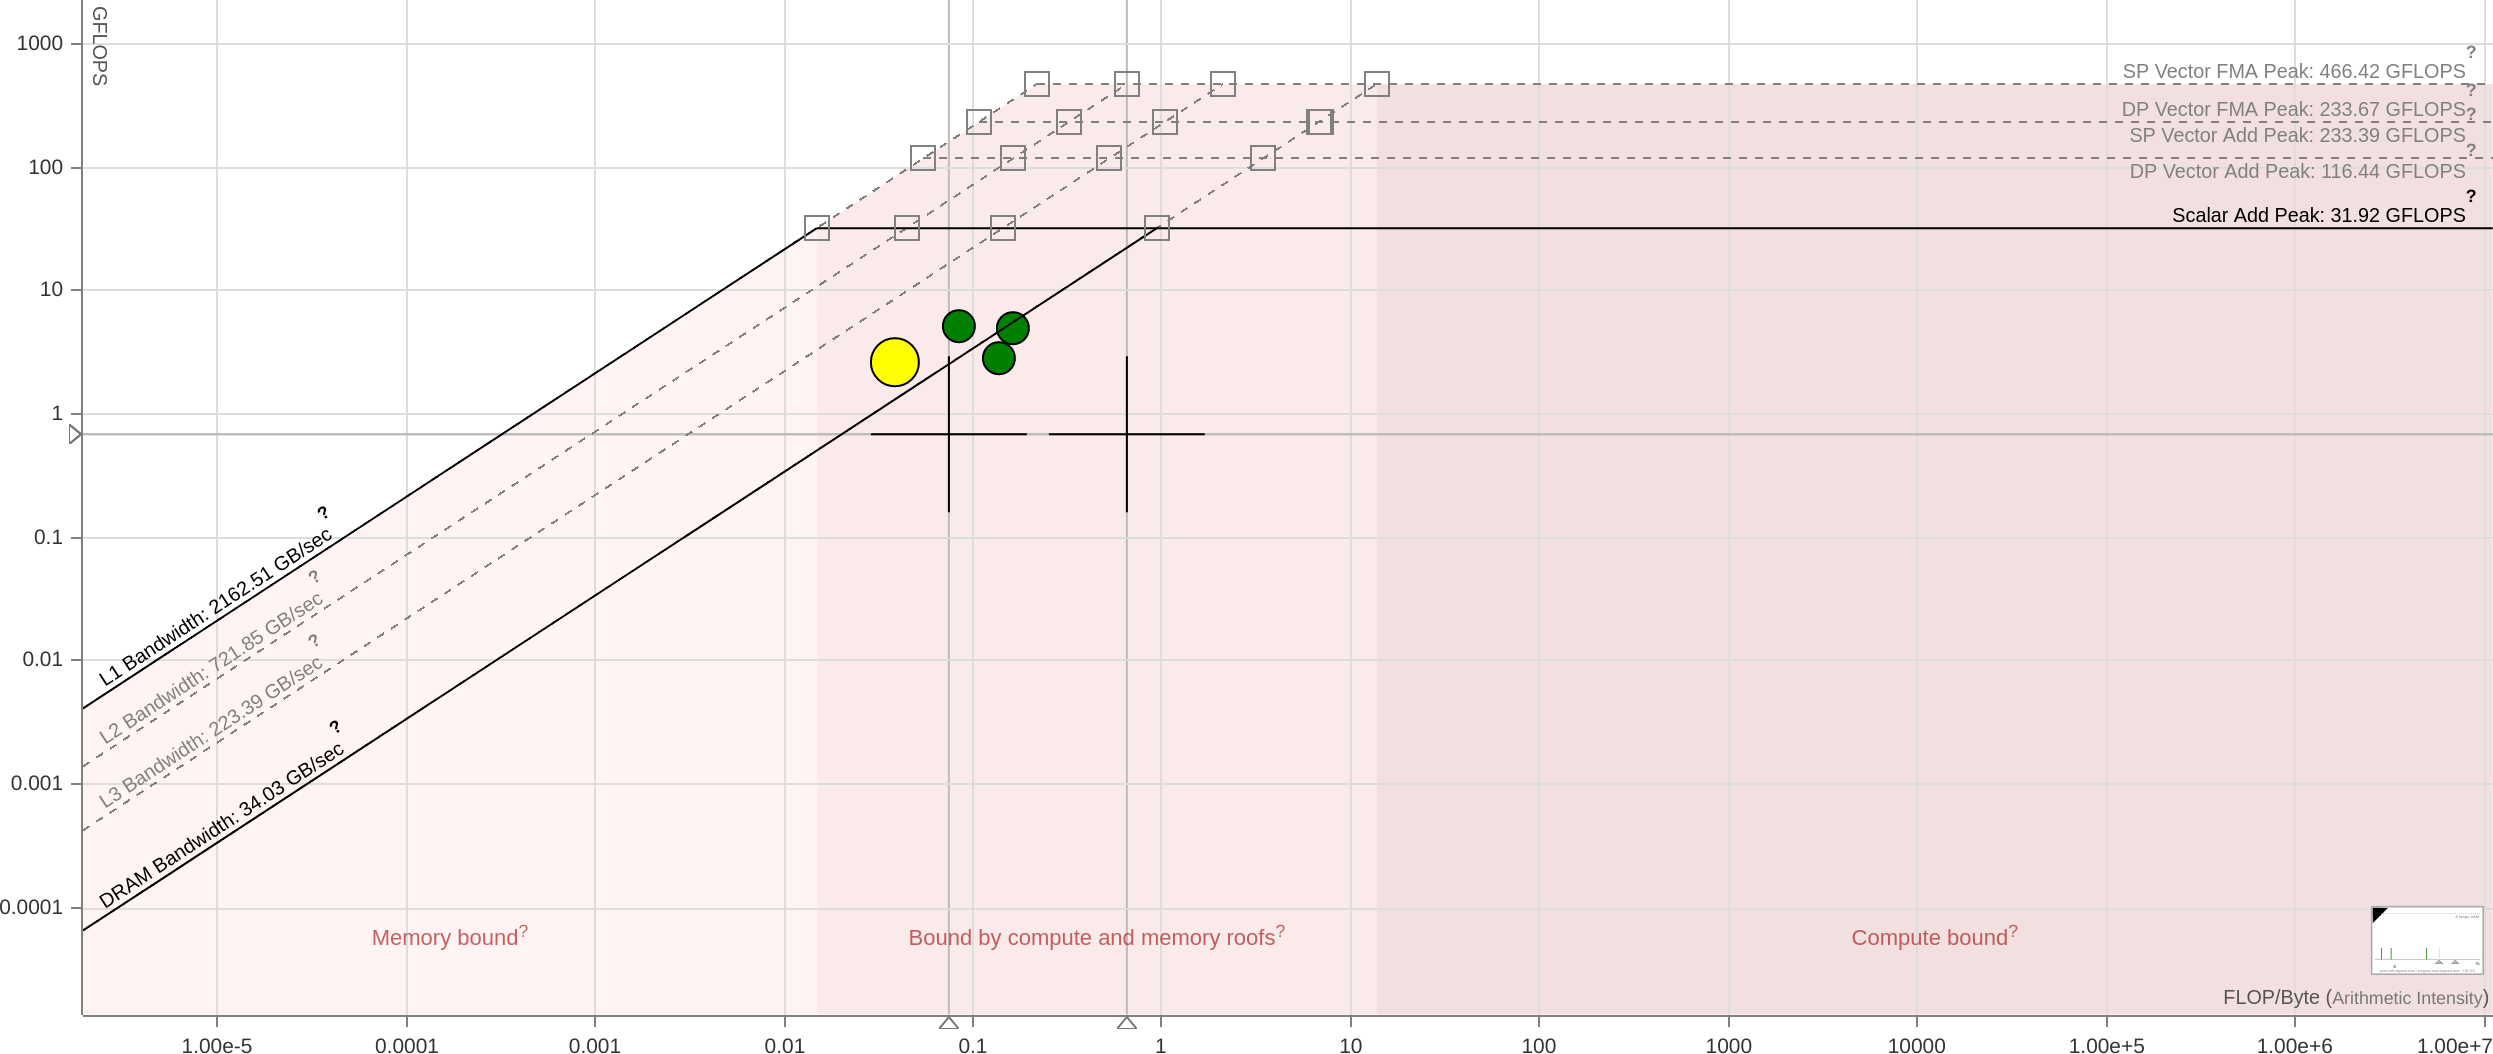
\includegraphics[width=\textwidth]{img/rooflines/roofline_p2p_95.png}
    \caption{\textit{Roofline model} del código \textit{point-to-point}, GCC}
    \label{fig:roofline_p2p_gcc}
\end{figure}

Por otro lado, para códigos compilados con GCC, con dispersiones del 90\% (\ref{fig:roofline_p2p_gcc_90}) y 99\% (\ref{fig:roofline_p2p_gcc_99}) se obtienen los modelos visibles en la Figura \ref{fig:rooflines_p2p_gcc_90_99}.

\begin{figure}[htpb]
    \centering
    \begin{subfigure}[b]{0.495\textwidth}
        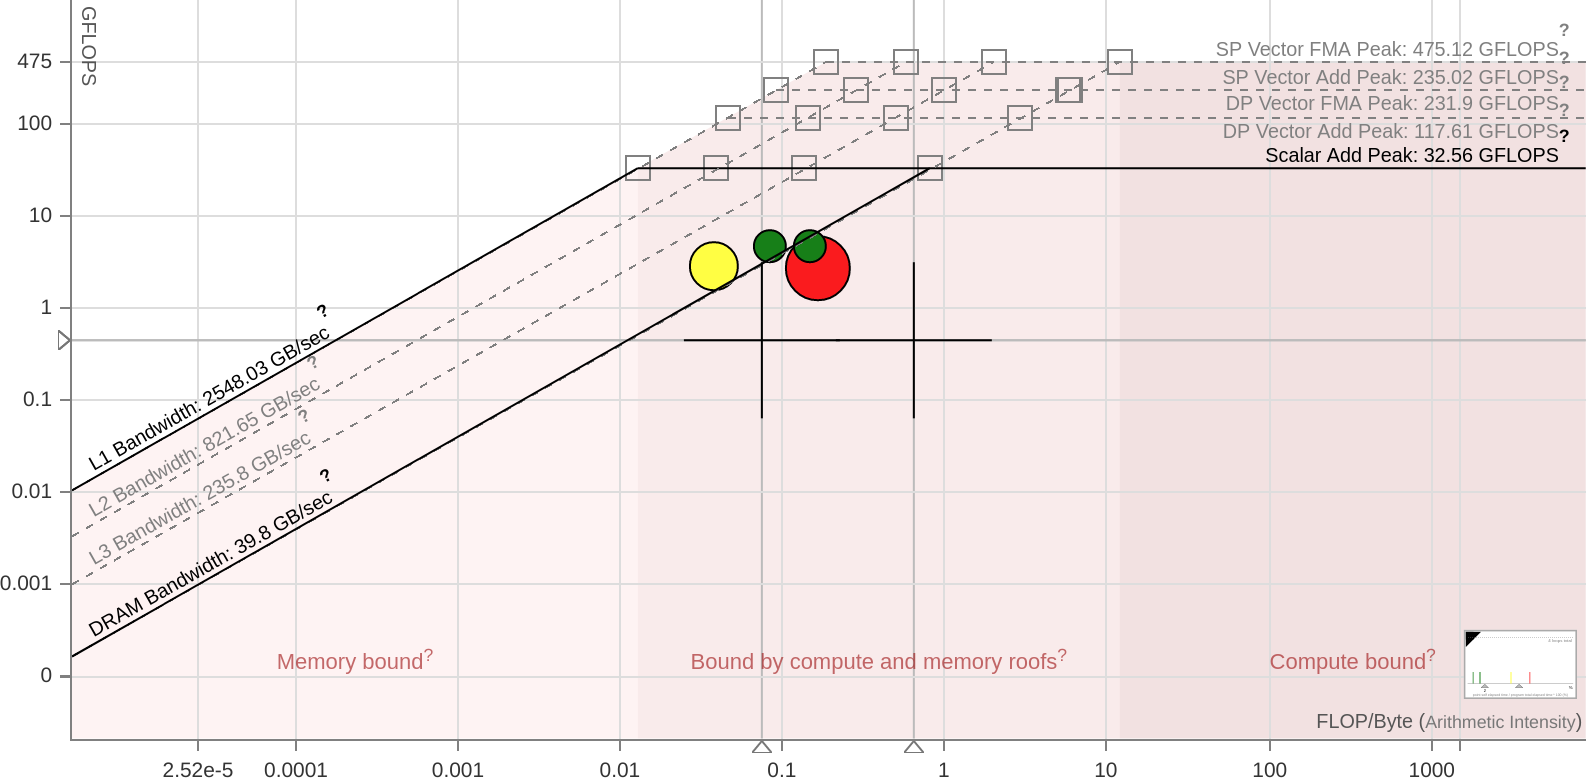
\includegraphics[width=\textwidth]{img/rooflines/roofline_p2p_90.png}
        \caption{\textit{Sparsity} del 90\%}
        \label{fig:roofline_p2p_gcc_90}
    \end{subfigure}
    \begin{subfigure}[b]{0.495\textwidth}
        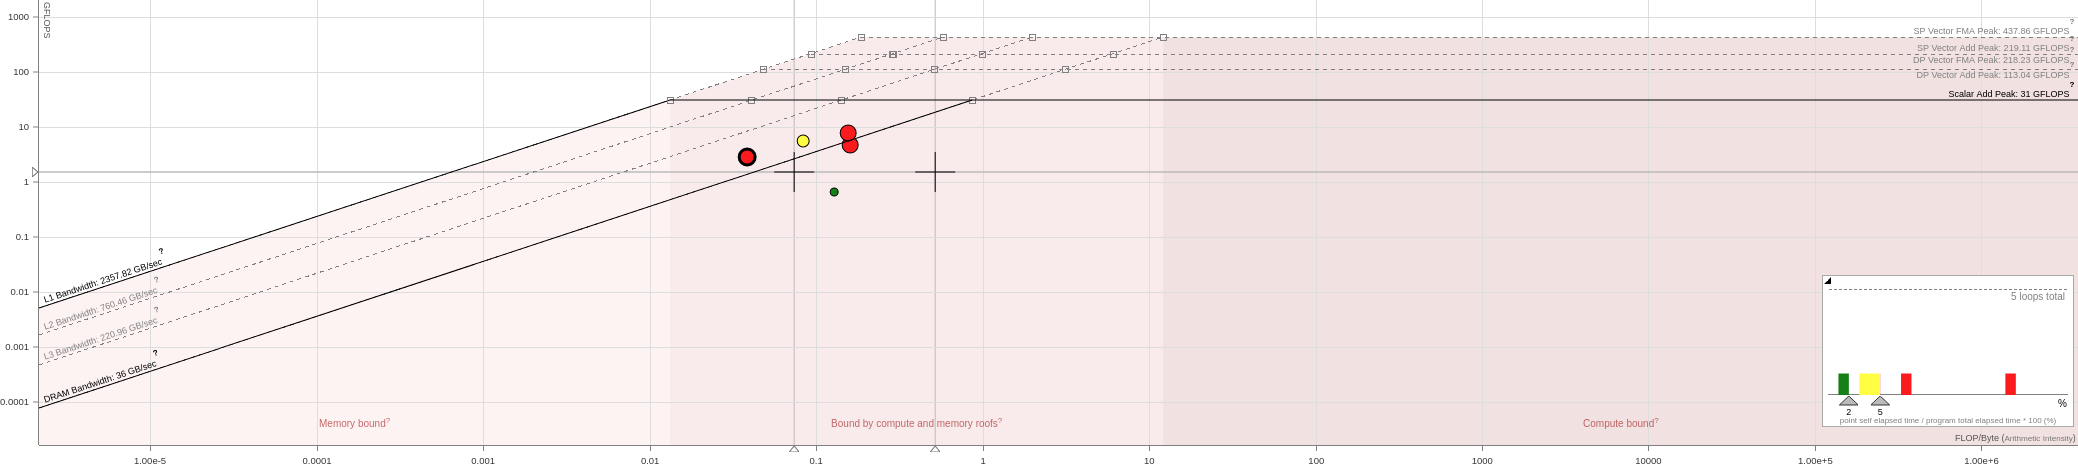
\includegraphics[width=\textwidth]{img/rooflines/roofline_p2p_99.png}
        \caption{\textit{Sparsity} del 99\%}
        \label{fig:roofline_p2p_gcc_99}
    \end{subfigure}

    \caption{\textit{Roofline models} de los códigos \textit{point-to-point}, GCC}
    \label{fig:rooflines_p2p_gcc_90_99}
\end{figure}

Y por último y como contraste, para las mismas redes al 99\% de índice de dispersión, se recopilan también los modelos de programas compilados con ICC (\ref{fig:roofline_p2p_icc_99}) e ICX (\ref{fig:roofline_p2p_icx_99}) en la Figura \ref{fig:rooflines_p2p_icc_icx_99}.

\begin{figure}[htpb]
    \centering
    \begin{subfigure}[b]{0.495\textwidth}
        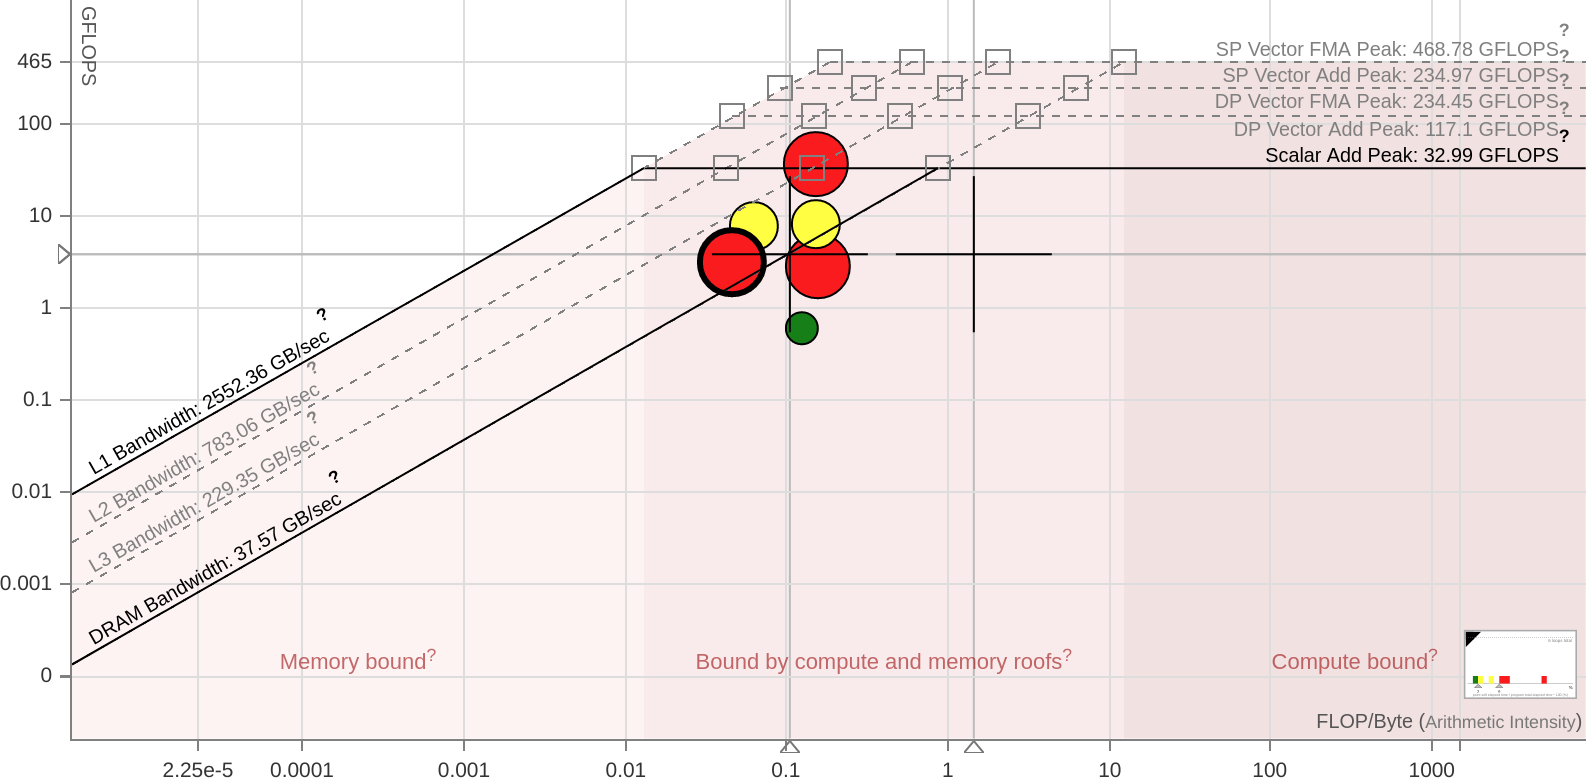
\includegraphics[width=\textwidth]{img/rooflines/roofline_p2p_99_icc.png}
        \caption{ICC}
        \label{fig:roofline_p2p_icc_99}
    \end{subfigure}
    \begin{subfigure}[b]{0.495\textwidth}
        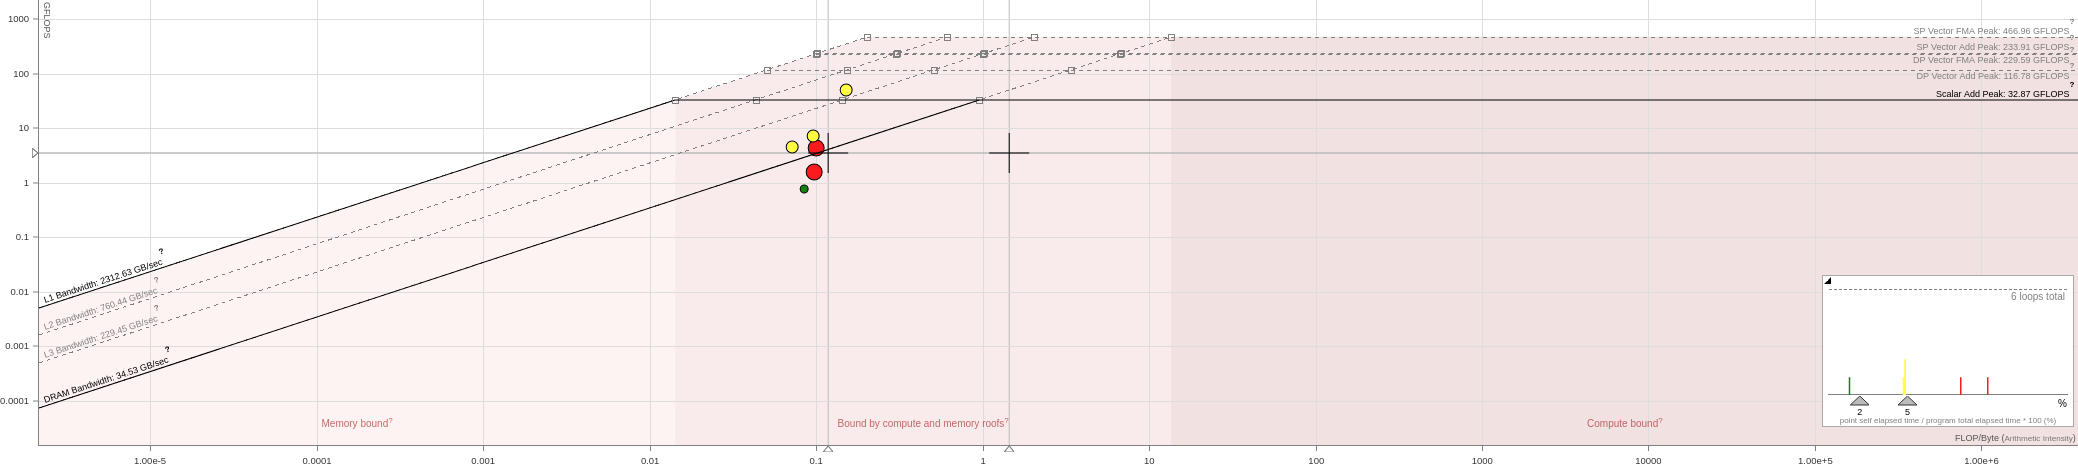
\includegraphics[width=\textwidth]{img/rooflines/roofline_p2p_99_icx.png}
        \caption{ICX}
        \label{fig:roofline_p2p_icx_99}
    \end{subfigure}

    \caption{\textit{Roofline models} de los códigos \textit{point-to-point} 99\% con ICC e ICX}
    \label{fig:rooflines_p2p_icc_icx_99}
\end{figure}

\section{Resultados}
Los resultados son cuanto menos sorprendentes. El rendimiento de \texttt{OpenBLAS} es fantástico, tal como se espera de una librería de dicha importancia. Por otro lado, \texttt{librsb} rinde particularmente mal. Esto indica que quizás esté pensada para niveles de dispersión varios órdenes de magnitud por encima de lo que se emplea en este trabajo, como por ejemplo para operaciones con matrices empleadas en redes sociales, con una muy elevada cantidad de ceros antes del primer decimal, para, por ejemplo, representar los usuarios que se siguen entre ellos.

Con respecto a los resultados de códigos punto a punto, los tiempos comienzan a superar a los obtenidos por \texttt{OpenBLAS} por encima del 87,5\% de dispersión. Esta \textit{sparsity} resulta algo elevada en el ámbito de las redes reuronales y deep learning, aunque todavía queda espacio para mejora mediante vectorización y, sobre todo, un correcto filtrado de lo datos de entrada para una mejor utilización de la memoria caché y una reordenación de operaciones más acertada por parte del compilador y otras posibles herramientas auxiliares (MACVETH).